\documentclass[
	msc,
	english
%% Para dissertações de mestrado, OU
%	mscproposta, %% Para propostas de dissertação de mestrado, OU
%	phd, %% Para teses de doutorado, OU
%	phdproposta, %% Para propostas de tese de doutorado
%	portugues %% Para documentos em português, OU
%	english %% Para documentos em inglês
]{ppgccufmg}

%\usepackage[brazil]{babel} %% se o documento for em português, OU
\usepackage[english]{babel} %% se o documento for em inglês
%\usepackage[latin1]{inputenc}
\usepackage{natbib}
\usepackage{xcolor}
\usepackage{lipsum}
\usepackage[
	colorlinks=true,
	linkcolor=blue, %% Cor dos links do sumário
	citecolor=red, %% Cor dos links das citações      
	urlcolor=magenta, %% Cor das urls
]{hyperref}
\usepackage{minted}
\usepackage{algorithm}
\usepackage{algpseudocode}

%% Exemplo de lista customizada ==================
%% Para criar uma lista customizada (como Lista de Algoritmos, Lista de Exemplos) que ficará juntamente com as Lista de Figuras e Lista de Tabelas, execute os 3 comandos abaixo substituindo "algoritmos" pelo tipo de lista que estará criando. Para adicionar a lista ao documento, deverá passar o seguinte parâmetro no comando \ppgccufmg:
%% \ppgccufmg{
%% 		...
%% 		listacustomizada={\listadealgoritmos}
%% }
% \newfloat[chapter]{algoritmo}{lol}{Algoritmo}
% \newcommand{\listaalgoritmosname}{Lista de Algoritmos} %% Título da lista
% \newlistof{listadealgoritmos}{lol}{\listaalgoritmosname} %% O primeiro parâmetro é o nome da lista, e este deverá ser passado no parâmetro listacustomizada={\nomedalista}
% \newlistentry{algoritmo}{lol}{0} %% Nome do ambiente de cada algoritmo, e.g., \begin{algoritmo} ... \end{algoritmo}

%% **** Caso não haja nenhuma lista adicional, os comandos acima podem ser apagados. ****
%% ===============================================

\newcommand{\yell}[1]{{\color{blue} [#1]}}
\newcommand{\tom}[1]{\yell{#1 --tom}}

\begin{document}
	\ppgccufmg{
		autor={Tomaz Gomes Mascarenhas}, %% Autor(a)
		titulopt={Demonstrando teoremas em Lean por meio da reconstrução de provas em SMT},
		tituloen={Proving Lean theorems via reconstructed SMT proofs}, %% Título em inglês
		cidade={Belo Horizonte},
		ano={2023},
		versaopt={Final},
		versaoen={Final}, %% Palavra que acompanhará 'Version' na folha de rosto em inglẽs
		orientador={Haniel Barbosa}, %% Para masculino
		fichacatalografica={fichacatalografica.pdf},
		folhadeaprovacao={folhadeaprovacao.pdf},
		resumo={resumo.tex}, %% Resumo em português
		palavraschave={Verifica\c{c}\~ao Formal, Lean, SMT},
		abstracten={abstract.tex}, %% Abstract em inglês
		keywords={Formal Verification, Lean, SMT}, %% Palavras-chave do abstract
		dedicatoria={dedicatoria.tex}, %% Arquivo .tex contendo a dedicatória
		agradecimentos={agradecimentos.tex},
		epigrafe={S\'o quem sonha acordado v\^e o sol nascer.},
		epigrafeautor={Unknown},
		% listadefiguras={sim}, %% Remova (ou comente) este parâmetro para remover a lista de figuras
		% listadetabelas={sim}, %% Remova (ou comente) este parâmetro para remover a lista de tabelas
		% listascustomizadas={\listadealgoritmos} %% Lista customizada (e.g., lista de algoritmos).
	}

	\chapter{Introduction}
	  \section{Context}
	    A mechanized proof is a proof, written in some language recognized by a computer, that had its validity checked by a trusted verifier. One of the main applications of these artifacts are formalizing mathematical theories. Indeed, there are well-known examples of successful formalizations. One of them is the mechanization of the proof of a theorem regarding Perfectoid Spaces\cite{scholze}, done by the fields-medalist mathematician Peter Scholze, together with the community of a system called Lean\cite{lean}. Scholze proved the theorem using pen and paper, but was unsure of the result due to its complexity. Once he translated the theorem and the proof to the language of Lean, the system could point out some mistakes he made, and, after fixing them, he could be sure of the correctness of the proof.

Another application of mechanized proofs is verifying the correctness of mission-critical software. Given a specification of the behavior of some program, the program is said to be correct if it respects the specification for any input it is given. For instance, one could specify that a sorting routine must always produce the sorted permutation of it's input list. In this case, a given sorting routine is said to be correct if it indeed produces the desired permutation, regardless of which list it receives. There are a variety of techniques to obtain correctness evidence for a software. The most common one is the development of tests. Besides being easy to write an efficient set of tests, there are many types of bugs that can be discovered with its execution. In fact, this approach is enough for a large amount of problems that are solved by software engineering. However, tests can’t guarantee that a program doesn’t have flaws, since the number of valid inputs is almost always exceedingly large, or infinite. This kind of guarantee is extremely important for mission-critical software, that is, systems that have critical responsibilities, such as the control of airplanes or medical equipment. In this context, one promising alternative is to use a mechanized proof of the correctness of the software as an evidence for its safety.

The process of generating mechanized proofs can be divided into
two categories: interactive and automatic.

Interactive theorem provers (ITPs) are mainly represented by proof assistants, in which, after defining
a theorem, the user attempts to manually write a proof for it,
relying on the tool to organize the set of hypothesis and
how the goal changed step-wisely through the proof, as well as to ensure the
correctness of each step according to a trusted kernel.
%
In order to keep the kernel simple and small (and, therefore, easy to be trusted), it's implementation usually just straightforwardly checks the logic rules from the logic implemented by the ITP.\ Because of this, each step must be explicitly stated by the user, making the tool costly to be used.
% %
% Each logic step must be explicitly stated by the user, which makes the tool
% costly to be used.

Automatic theorem provers (ATPs), on the other hand,
only require the user to define a conjecture, proceeding automatically to
determine whether there exists a proof for it, or possibly providing a
counter-example if it can find one.
%
Although they are easier to use, ATPs require a large
codebase to implement all the algorithms necessary to execute the search for a proof,
making them more susceptible to errors and harder to be trusted.
One possible way to overcome this trust issue is to produce
a mechanized proof verifying the correctness of the ATP, however,
besides being a very complex task, once the proof is done the
development of the ATP becomes freezed, otherwise it would
have to be verified again.

Another approach to increase the confidence in ATPs is to have them provide a
proof to support their results, so that it can be independently verified whether
it indeed proves the theorem in question. This has the downside of creating a need
for allocating resources to verify the proof of every single theorem that is proved.
On the other hand, as long as the proof format doesn't change, the implementation
of the solver can be modified without requiring a modification in the checkers. Also,
it is important to consider that it is often simpler to verify proofs than to verify
the tool itself.

Another important advantage of the second approach is that it allows the ITPs to leverage the automatic proving performed by the ATPs by using the proofs they produce, since the requirement for accepting a proof, i.e.\ that each step is correct to its internal logic,
can be applied to the ATP proof.
%
By connecting these systems, it would be possible for the user of the ITP to focus on more complex steps of the proof, such as defining an induction hypothesis, while delegating the burden of other long and straightforward steps to the ATP.\ Indeed, this
connection is so important that there are projects like Hammering Towards QED~\cite{hammering}
that outline all the efforts that were already made in order to integrate
interactive and automatic theorem provers. In this paper, the authors describe in detail each component that a system that creates a connection between ATPs and ITPs has to implement, as well as the main issues that they have to solve, based on existing programs that were successful in this task. Besides that, they show their potential through several large benchmarks. 


	  \section{Contributions}
	    Given this context, we present a set of tools that would be an essential
part of the integration between the ITP Lean 4~\cite{lean} and the SMT solver cvc5~\cite{cvc5}.
%
Specifically, we aim to build a system that takes proofs of the unsatisfiability of
SMT queries produced by cvc5 and reconstructs them in Lean.
%
The main motivation of this project is that despite the fact that Lean is
emerging as a promising programming language and proof assistant and being
widely used by mathematicians in large-scale
formalizations~\cite{mathlib, scholze}, there is currently no way to
interact with SMT solvers from it, even though these systems have been
central in previous developments of proof automation in ITPs, as we will show in Sections~\ref{sec:smtcoq}
and~\ref{sec:sledgehammer}. The contribution of the present work
would enable a faster development of this kind of project using Lean.

We use the cvc5 solver because it already has a module for exporting proofs as
Lean scripts~\cite{Barbosa2022}, using a representation of the SMT terms\footnote{For more details
about the SMT term language, see SMT-LIB~\cite{smtlib}.} as an inductive type in Lean.
However, these proofs are not fully verified by Lean's checker. Instead, a set of
axioms are declared in Lean, representing all the logical rules that cvc5 uses to prove
theorems, and the ITP only checks whether the rules were applied correctly and whether
the end result of applying all the rules in the proof is, indeed, the required one.
Our main contributions are to eliminate the need of increasing the trusted base by introducing
those axioms and to make the proofs operate over native Lean terms, as opposed to terms
of the inductive type that represents SMT terms.

Note that the set of tools we are proposing does not implement the full integration
between Lean and cvc5. For instance, we do not implement a module for translating
Lean goals into an equivalent SMT problem. However, our project is being used
as part of the joint project Lean-SMT\footnote{The code for the project can be found at \url{https://github.com/ufmg-smite/lean-smt}}, that aims to implement a tactic in Lean
that would perform the complete process, that is, starting from a Lean goal, translating it to a SMT query, invoking a solver to try to prove it and lifting the proof produced (in case it is found) to Lean's language, so that it can be used as a proof for the original goal.

	  \section{Related Work}
	    \subsection{Hammering Towards QED}
           \label{sec:hammering}
			\label{sec:hammering}
As previously mentioned, Hammering Towards QED is a project
that aims to describe all the tools, which the paper calls ``hammers'',
that were created with the purpose of connecting automatic and interactive
theorem provers. Besides that, this document also outlines
the main components that such tools usually have. They are
the following:

\begin{itemize}
  \item The premiss selection module: that identifies
        a subset of the facts previously demonstrated in the
        ITP that are more likely to be useful in order to
        prove the given goal, to be dispatched to the ATP.\@
  \item The translation module: that builds a problem in the language of the
        ATP that corresponds to the original goal from the ITP and using
        the premisses that were selected.\@
  \item The proof reconstruction module: that lifts the proof produced
        by the ATP into a proof that is accepted by the ITP.\@
\end{itemize}

In our case, we will restrict ourselves to implement a proof reconstruction module.
The three main strategies used to reconstruct the proof produced
by the automatic system inside the interactive one are also described in the paper.

The first one is to use the ITP to verify a deeply embedded version of the proof
received, and, in case it is succesful, reflect this proof inside it's checker, proving
the original goal. More specifically, the hammer defines a datatype to represent
terms in the ATP and a set of functions to manipulate values on those datatypes, representing
the axioms that the solver uses to transform the terms. Then, a lifting function is defined, that is,
a function that take a value of this datatype and outputs an equivalent term in the native
language of the ITP.\ Finally, the correctness of each transformation function is
verified with respect to the lifting function, in the sense that, if the input term
was lifted to a value that is provable in the ITP's logic, then the output term will
also be provable. The ATP's proof will be represented as a sequence of those
transformations, and their correctness are proved \textit{a priori}. When checking
a specific proof, the only step that the ITP must perform is to compute the result
of the application of all the functions in the solver's output, and to check if
the final term matches with the expected one. This technique is known as
the Certified approach\ \cite{snipe}.

The second one is to match each axiom in the ATP's logic into a proved lemma or a tactic
\tom{is it okay to use tactic here? should I introduce the term first?}
defined in the ITP that works directly with native terms of the system.
The proof produced by the automatic solver is then parsed into a sequence of applications
of those lemmas and tactics and replayed inside the ITP.\ In this case, the proof is built
on the fly and does not have it's correctness guaranteed (it can fail in the middle of the
proccess in case the ATP or the hammer did something wrong). On the other hand,
this technique skips computations done over embedded terms, which have to be done by the
Certified approach, having the potential to have a better
performance. This approach is known as the Certifying approach\ \cite{snipe}.

The third one is to compile the proof into the ITP's source code. This implies generating
an actual script in the native language of the interactive system
that corresponds to the proof received. After the script is generated, it is
possible to postprocess\tom{maybe copy the references that hammering towards use to talk about this?}
it in order to make the proof easier to be checked,
in a way that the final script can possibly ignore a large portion of the
original proof. This approach can be inconvenient for very large proofs,
as it requires that the script is stored in some filesystem. However,
it has the advantage over the two previous methods of only requiring access to the ATP
on the first time that the proof is checked.

In this project we will be using the second approach. We give more details about this
decision in the later chapters.

	    \subsection{SMTCoq}
           \label{sec:smtcoq}
			One notable example of such integrations is SMTCoq~\cite{smtcoq}.
It is a plugin for the proof assistant Coq~\cite{Bertot2004} that
can be used as a tactic to prove theorems via their encoding into
SMT and by lifting proofs produced by the SMT solvers veriT~\cite{Bouton2009}
and CVC4~\cite{Barrett2011}. The tool relies on a preprocessor written in OCaml
to transform proof witnesses coming from different solvers into certificates in
the Coq language. The system has a set of checkers for each theory in SMT, each
one of them consisting of theorems asserting the validity of certain transformations
in the SMT terms. All those checkers are connected by the main checker, that
is essentially a theorem stating that if all the transformations resulted in an
empty clause, then the lifting of the original term is false, for any instantiation
of its free variables. This kind of reasoning is known as proof by computational
reflection~\cite{reflection} which is an instance of Certified Transformations, which will be described
in Section~\ref{sec:certifiedVsCertifying}.

		\subsection{Sledgehammer}
           \label{sec:sledgehammer}
			The ITP Isabelle/HOL~\cite{Nipkow2002} has a similar tool,
namely, Sledgehammer~\cite{sledgehammer}. This system achieves its goal by
invoking several SMT solvers in parallel to prove a given goal and collecting
their output to determine which lemmas must be applied in order to prove the theorem
inside Isabelle. In a way, this approach is very similar to the one we're using in this project, as the proof is produced on
the fly (known as the Certifying approach, which will also be described in Section~\ref{sec:certifiedVsCertifying}) as opposed
to having a single theorem that establishes once and for all
that, if all steps performed by the solver were successful,
then the original goal is valid, as is done by SMTCoq.

	  \section{Organization of this document}
	    In Chapter~\ref{chap:formalPrelim} we present the concepts involved in our work.
We describe the SMT problem in detail, as well as the main techniques used to solve
it and the proof certificates produced by cvc5. We also present Lean and give
an overview of the features of the language we have employed throughout the project.
%
Then, in Chapter~\ref{chap:certified}, we describe the steps necessary to implement
the reconstruction of proofs from cvc5 in Lean using the approach of certified
transformations.
%
Next, in Chapter~\ref{chap:rcons}, we present in detail our implementation of the
reconstruction using the certifying transformations approach.
%
This implementation is evaluated in Chapter~\ref{chap:eval}.
%
Finally, we present some possible directions for future work in
Chapter~\ref{chap:future}.

	\chapter{Formal Preliminaries}
	  \section{Satisfiability Modulo Theories}
	    \subsection{Description of the Problem}

The Boolean Satisfiability Problem (SAT) consists of, given a formula in Propositional Logic (PL) containing free variables, determine whether exists a function that assigns each variable to a boolean value, in a way that, after replacing the variables by their values provided by the function, the formula is evaluated to \textit{true}. We say that a formula is satisfiable if such function exists, and unsatisfiable otherwise. In this work, we will be focusing on the problem CNF-SAT, an equivalent version of SAT in which the input formula always comes in Conjuctive Normal Form, that is, a conjunction of disjunctions. From now on, we will use SAT to refer to the CNF-SAT problem. Besides that, we will use the name \textit{clause} to refer to one of the disjunctions in some input formula for SAT.

Satisfiability Modulo Theories (SMT)~\cite{smt} is a generalization of SAT.\ There are two additions in this version of the problem: the first one is that the input formula can contain quantifiers binding variables, which will affect the satisfiability of that formula. Therefore, any formula in First Order Logic is a valid input to the SMT problem. The second addition is the inclusion of a set of theories that allows the problem to refer to variables of different domains. More precisely, a theory consists of a sort (for instance, integers) over which a subset of the variables of the problem can range over and a set of symbols that represents operations over these sorts with predefined semantics (for instance, addition and comparison operations). Note that SMT problems are allowed to use multiple theories in the same instance. The logic framework that corresponds to Propositional Logic with these two additions is known as Many-Sorted First Order Logic (MSFOL). The semantics of this logic is given in detail in~\cite{many_sorted}. In the next section we give a brief overview of it.

% EXAMPLE -- remove?

% For instance, let $x$ and $y$ be integer variables and the symbols $+$ and $<$ have their usual meaning of addition and comparison of integers. Then, consider the formula:

% \begin{center}
%   $0 < x \land x < 2 \land (\forall z . (y < z) \lor x + y < 1 + y)$
% \end{center}

% By the first two propositions we can derive that $x = 1$. But if $x = 1$ then $x + y$ can't be lesser than $1 + y$. Also, it is impossible to choose a value for $y$ such that $\forall z . (y < z)$. Therefore, there is no value for $x$ and $y$ that would satisfy the whole formula. In other words, it is unsatisfiable. On the other hand, the following formula is satisfied by assigning, for instance, $x = 0$ and $y = 3$:

% \begin{center}
%   $-1 < x \land x < 1 \land (\forall z . (y < z) \lor x + y < 1 + y)$
% \end{center}

% END EXAMPLE

% tem que falar o que eh uma demonstracao nesse contexto antes de falar isso
% Some of the most relevant theories in SMT are Linear Integer Arithmetic (LIA), Linear Real Arithmetic (LRA), Bitvectors (BV) and Equality and Uninterpreted Functions (EUF).
% In this work, we will focus on reconstructing proofs from LIA, LRA, EUF and regular SAT proofs of unsatisfiability.

\subsection{Applications}

Given a program and a formal specification of some property related to the program, it is often \tom{always?} the case that we can express the proposition that asserts that the program satisfy the property as an SMT instance. For instance, consider the well known \textit{abs} function, that takes an integer and returns its absolute value. The usual way to implement it is through a branch that checks whether the input variable is positive or negative. In case it is positive, its own value is returned. Otherwise, the value multiplied by $-1$ is returned:

\begin{algorithm}
\caption{Original Absolute Function}~\label{originalAbs}
\begin{algorithmic}
\Function{abs}{x}
\If{$x < 0$}
  \State\Return$-x$
\Else
  \State\Return$x$
\EndIf
\EndFunction
\end{algorithmic}
\end{algorithm}

In program analysis, it is quite useful to eliminate branches from programs since this action completely removes one possible path that the flow of the program can take (besides optimizing it's performance). Obviously, this operation must be done with caution to not modify the original behavior of the program. In his book~\cite{hacker_delight}, Henry Warren proposes an alternative implementation for the \textit{abs} function which doesn't have branches:

\begin{algorithm}
\caption{Branchless Absolute Function}~\label{branchlessAbs}
\begin{algorithmic}
\Function{abs'}{x}
  \State $y \gets x >> 31$
  \State \Return $(x \bigoplus y) - y$
\EndFunction
\end{algorithmic}
\end{algorithm}

Where $\bigoplus$ represents the bitwise xor operation. We can design an instance of the SMT problem that asserts that both implementations produce the same output, when given the same input. We present the instance written in SMT-LIB~\cite{smtlib}, a standardized syntax for representing SMT problems:

\begin{minted}[linenos]{smtlib2.py -x}
(set-logic QF_BV)
(declare-const x (_ BitVec 32))
(declare-const result1 (_ BitVec 32))
(assert (= result1 (ite (bvslt x #x00000000) (bvneg x) x)))
(declare-const y (_ BitVec 32))
(declare-const result2 (_ BitVec 32))
(assert (= y (bvashr x (_ bv31 32))))
(assert (= result2 (bvsub (bvxor x y) y)))
(assert (distinct result1 result2))
(check-sat)
\end{minted}

First, we set the combination of theories that will be used in this problem. In our case, we will be using \textit{QF\_BV}, which stands for quantifier free bitvectors. This means that this instance of the problem is not allowed to use quantifiers and is allowed to declare and use variables living in the Bitvector sort, as well as operations over this sort. Bitvectors are fixed-length arrays of bits. They are useful for representing machine integers, as they can simulate their semantics.

Next, in lines 2 and 3, we define two constants, both from the sort \textit{BitVec 32} (arrays of 32 bits): \textit{x} and \textit{result1}. The first one represents the input value from the original \textit{abs} function, and the second one, the result produced by that function. We then have to add an assertion in line 4 that binds the variable \textit{result1} to the output of the function \textit{abs} in terms of \textit{x}. We translate the branch from the pseudocode as the \textit{ite} operator, the comparison as the \textit{bvslt} operator and the multiplication by -1 as the \textit{bvneg} operation. This assertion will be encoded as a regular implication from SAT, where the premiss is it's proposition and the conclusion is the rest of the problem, which still needs to be defined. In lines 5 to 8 we repeat the process to define \textit{y} and \textit{result2}, which corresponds to the result of the branchless \textit{abs} function. Finally, we assert that \textit{result1} and \textit{result2} must be different in line 9. If this problem is satisfiable, then there is a value for \textit{x} which produces different values in each function. If it is unsatisfiable, then we can be sure that no such value exists, therefore, both functions are equivalent. Note that we are not verifying that the actual code of the functions are equivalent, just an abstraction over it's implementation.

% Given that we have very efficient systems to solve such problems, which will be introduced later, the possibility of formally verifying programs using this technology is quite promising. Indeed, \tom{pegar referencias do paper do leonardo (https://fm.csl.sri.com/SSFT14/smt-application-chapter.pdf)}
%

% \begin{itemize}
%   \item revolucao sat
%   \item representar propriedades de programas como problemas smt
%   \item geracao de casos de teste
%   \item geracao de programas
%   \item F*, Dafny
% \end{itemize}

\subsection{Many-Sorted First Order Logic}

define formarly many sorted first order logic

talk about fixing the meaning of some theories to improve performance

skipping this for now, I will write the rest of the thesis so I have a better understanding of what needs to go here

\subsection{SMT Solvers}

A SMT solver is a piece of software whose main goal is to solve the SMT problem. Many-Sorted First Order Logic is undecidable in it's most general form~\cite{fol_undec}, therefore SMT solvers have to limit themselves to use heuristics to solve the largest possible subset of instances of the problem. In this section we present the ideas used by these systems that are most relevant to the present work.

\subsubsection{DPLL}

First, let’s explore how SAT is solved. Although MSFOL is not decidable, Propositional Logic is, therefore, it is possible to design a decision procedure for SAT.\@ Indeed, one simple way to check whether a formula in PL with $n$ variables is satisfiable or not is to simply test each one of the $2^{n}$ functions assigning truth values to those variables.

A more efficient alternative of a decision procedure for PL is the DPLL algorithm~\cite{dpll}. DPLL is based on the \textit{Resolution} theorem:

\begin{theorem}[Resolution]
Let $x$ be a literal. Let $C_{1}$ and $C_{2}$ be two clauses such that $x \in C_{1}$ and $\overline x \in C_{2}$. Then $C_{1} \wedge C_{2} \rightarrow (C_{1} \setminus x) \vee (C_{2} \setminus \overline x)$.
\end{theorem}

More specifically, it is based on \textit{Unit Resolution} (UR), that is, a more specific version of Resolution in which $C_{1} = \{x\}$ or $C_{2} = \{\overline x\}$. We present it's pseudocode:

\begin{algorithm}[H]
\caption{DPLL Algorithm}~\label{dpllAlgo}
    \hspace*{\algorithmicindent} \textbf{Input:} $\psi$, a formula in CNF \\
    \hspace*{\algorithmicindent} \textbf{Output} \textit{true} or \textit{false}, depending whether $\psi$ is satisfiable
\begin{algorithmic}
\Function{DPLL}{$\psi$}
\If{$\exists C \in \psi .\, C = \{\bot\}$}
  \State~\Return~\textit{false}
\ElsIf{$\forall C \in \psi .\, \top \in C$}
  \State~\Return~\textit{true}
\Else
  \If{$\exists x \in Vars(\psi) \,$ such that $x$ is a target for UR}
    \State $\langle C_{1}, C_{2} \rangle \gets$ \Call{findClauses}{$x$} \Comment{Clauses suitable for applying UR with $x$}
    \State~\Return~DPLL($\psi \cup C_{1} \diamond C_{2}$)
  \Else
    \State~Let $x$ be an unassinged variable in $\psi$
    \State~\Return~\Call{DPLL}{$\psi_{\{x \gets \top\}}$} $\vee$ \Call{DPLL}{$\psi_{\{x \gets \bot\}}$}
  \EndIf
\EndIf
\EndFunction
\end{algorithmic}
\end{algorithm}

The algorithm works as follows: first, it checks to see if the formula can be evaluated to \textit{true} or \textit{false}. In case it can't, the procedure finds as many variables in which it can apply Unit Resolution as possible. Once there are no more possibilities, it chooses an arbitrary variable and make two recursive calls: one assigning this variable to \textit{true} and the other one to \textit{false}. Since these are the only two possibilities for that variable, the input formula is satisfiable if and only if one of the recursive calls returned \textit{true}. The algorithm uses this information to simply return the disjunction between the two return values.

\subsubsection{Congruence}


\subsection{Proofs in cvc5}

	  \section{Lean's Type Theory}
	    take a look at chapter 2 of smtcoq
	    \begin{itemize}
	      \item Falar sobre porque eh facil confiar no proof assistant
		  \item Explicar que taticas extendem a linguagem mas nao aumentam o trusted core
	    \end{itemize}
	  \section{Lean's Framework for Metaprogramming}
	\chapter{Certifying Reconstruction of SMT Proofs in Lean}
	  \section{Certified vs Certifying}
      \label{sec:certifiedVsCertifying}
	  \section{Classical vs Intuitionist (?)}
	  \section{Tactics}
	  \section{The Complete Architecture}
	  \section{Skipping the Parser}
	  % maybe think of other optimizations and make a section about this
	\chapter{Evaluation}
	\chapter{Future Work}

	% \chapter{Introdução}
	% 	a introducao vem aqui
	% \chapter{Desenvolvimento}
	% 	\lipsum[1-4]

	% 	\begin{algoritmo}
	% 		\centering
	% 		\framebox[.5\textwidth]{\texttt{Código, Código, Código}}
	% 		\caption{Este é o meu Algoritmo 1.}
	% 		\label{alg:algoritmo1}
	% 	\end{algoritmo}

	% 	\begin{algoritmo}
	% 		\centering
	% 		\framebox[.7\textwidth]{\texttt{Mais Código, Mais Código, Mais Código}}
	% 		\caption{Este é o meu Algoritmo 2.}
	% 		\label{alg:algoritmo2}
	% 	\end{algoritmo}

	% 	\begin{figure}[h]
	% 		\centering
	% 		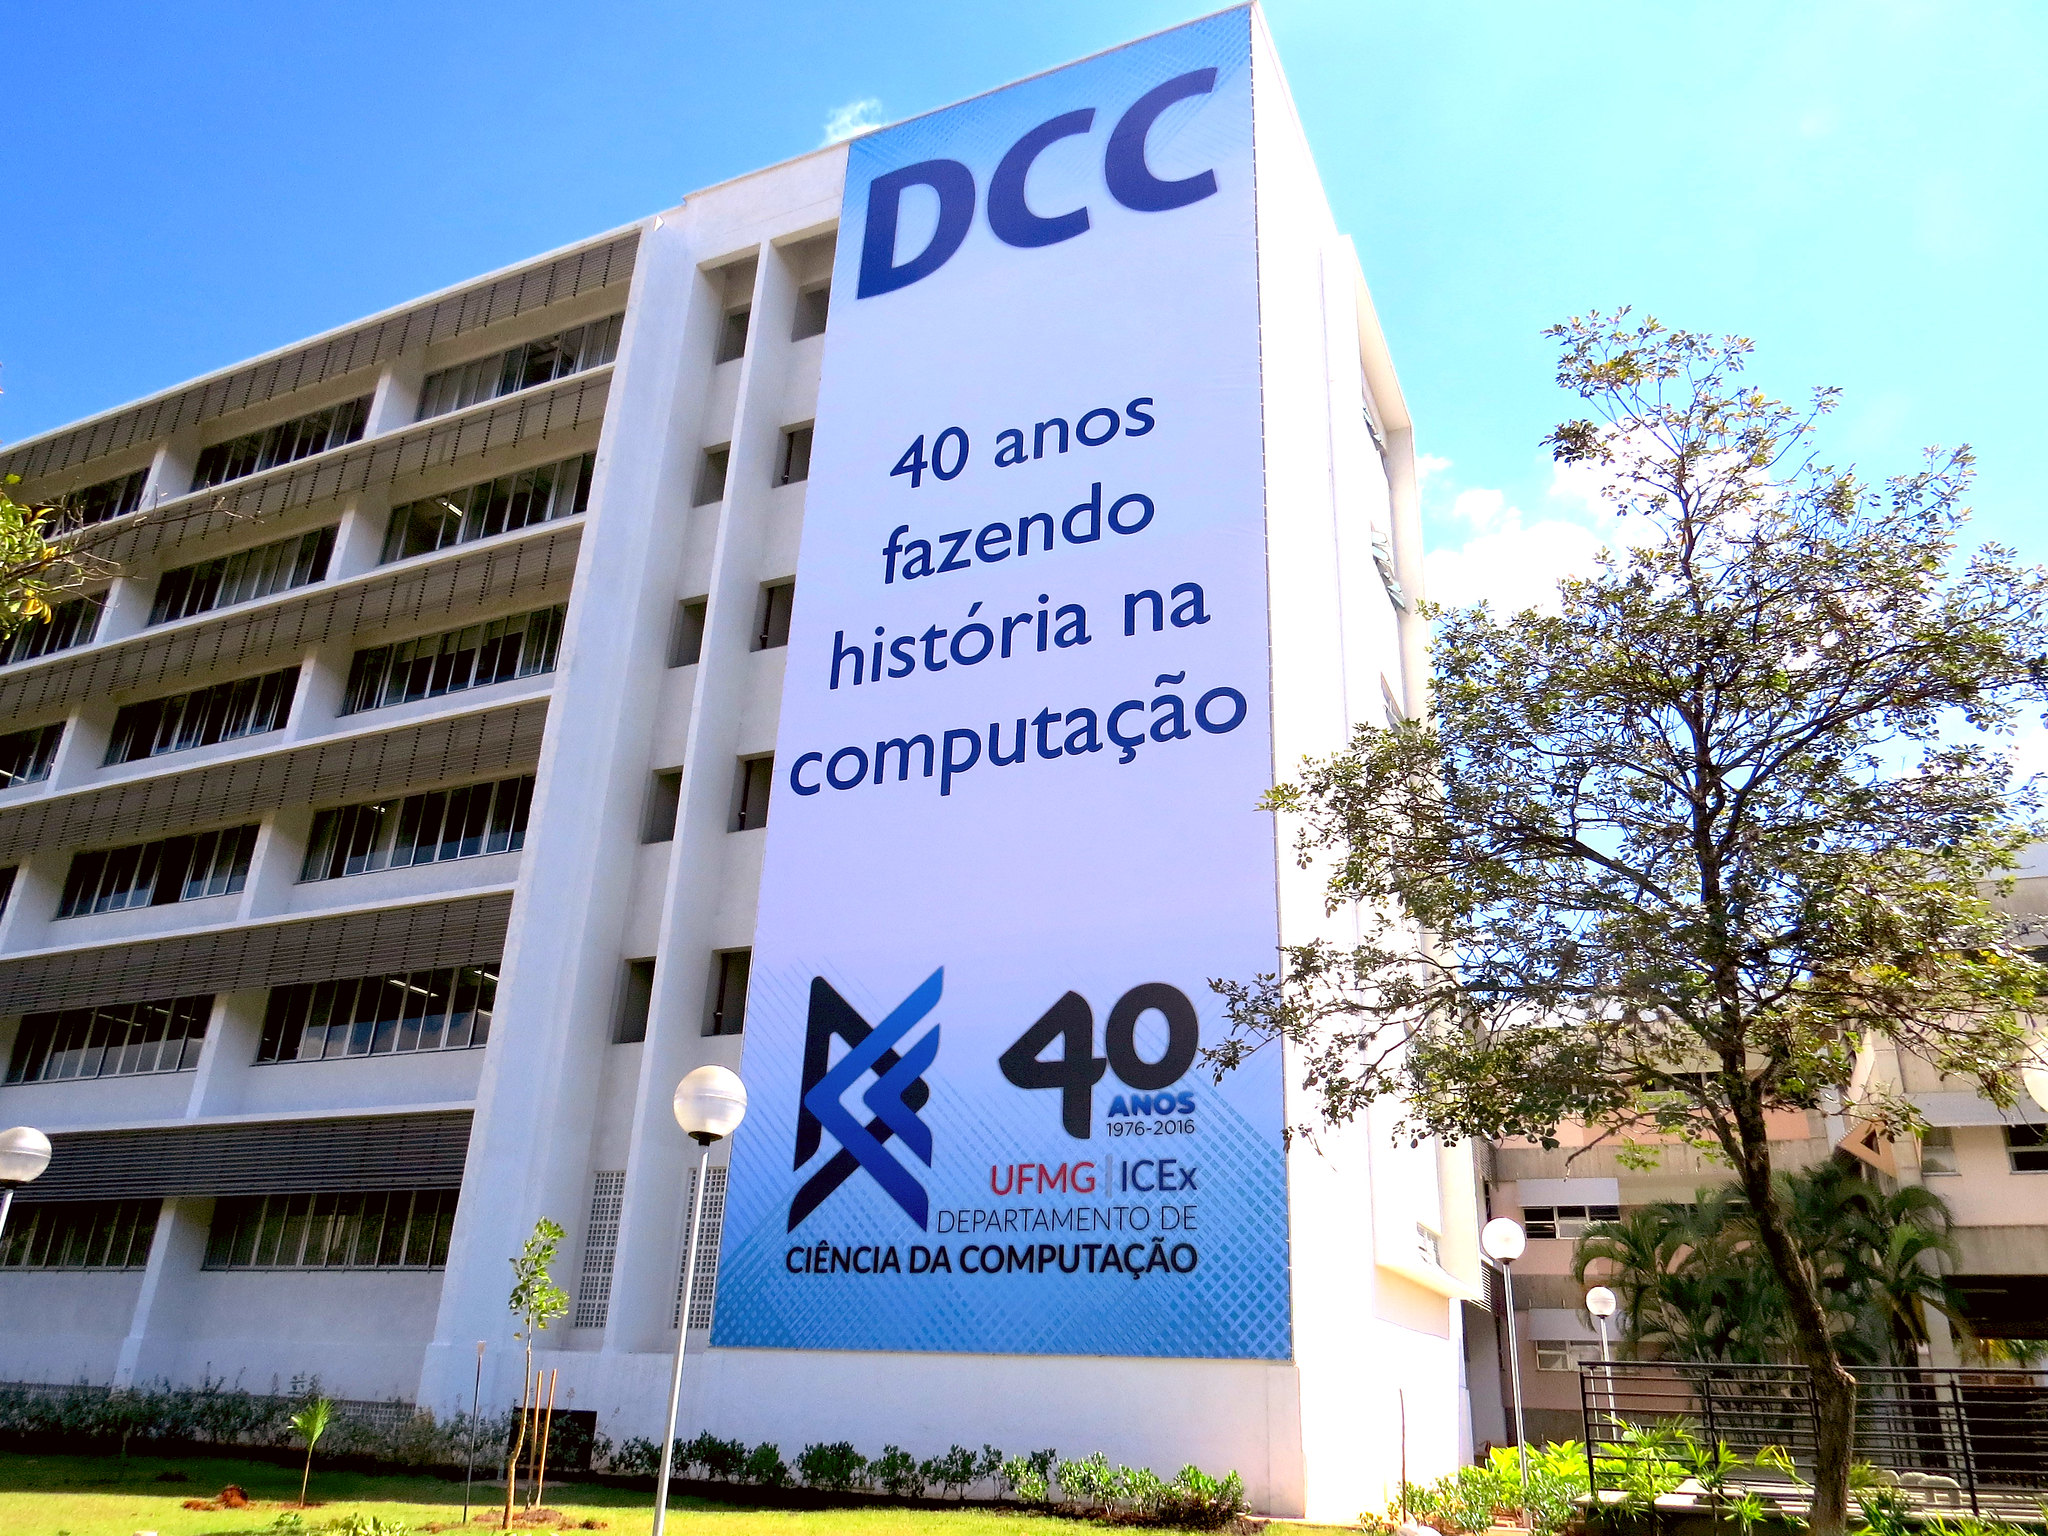
\includegraphics[width=\textwidth]{img/dcc.jpg}
	% 		\caption{Prédio do DCC em 2016.}
	% 		\label{fig:exemplo}
	% 	\end{figure}

	% 	\lipsum[5]

	% 	\begin{table}[h]
	% 		\centering
	% 		\begin{tabular}{c|ccccccccl}
	% 			Natural & \multicolumn{9}{c}{Real}   \\ \hline
	% 			1 & 0.  & {\color{red} 2}  & 3   & 6   & 4   & 3   & 6   & 7   & $\ldots$ \\
	% 			2  & 0.  & 0   & {\color{red} 9}  & 8   & 4   & 7   & 3   & 2   & $\ldots$ \\
	% 			3  & 0.  & 1   & 9   & {\color{red} 3}  & 2   & 1   & 4   & 0   & $\ldots$ \\
	% 			4  & 0.  & 8   & 4   & 3   & {\color{red} 2}  & 7   & 9   & 2   & $\ldots$ \\
	% 			5  & 0.  & 0   & 1   & 2   & 9   & {\color{red} 3}  & 4   & 8   & $\ldots$ \\
	% 			6  & 0.  & 2   & 8   & 2   & 6   & 5   & {\color{red} 8}  & 3   & $\ldots$ \\
	% 			7  & 0.  & 0   & 2   & 1   & 5   & 3   & 7   & {\color{red} 4}  & $\ldots$ \\
	% 			$\vdots$ & $\vdots$  & $\vdots$  & $\vdots$  & $\vdots$  & $\vdots$  & $\vdots$  & $\vdots$  & $\vdots$  & $\ddots$ \\ \hline
	% 			\multicolumn{1}{l|}{} & \multicolumn{1}{l}{0.} & \multicolumn{1}{l}{{\color{red} 2}} & \multicolumn{1}{l}{{\color{red} 9}} & \multicolumn{1}{l}{{\color{red} 3}} & \multicolumn{1}{l}{{\color{red} 2}} & \multicolumn{1}{l}{{\color{red} 3}} & \multicolumn{1}{l}{{\color{red} 8}} & \multicolumn{1}{l}{{\color{red} 4}} & $\ldots$
	% 		\end{tabular}
	% 		\caption{Cantor: Existem infinitos diferentes!}
	% 		\label{tab:exemplo}
	% 	\end{table}

	% 	\section{Usando referências}
	% 		Segundo \cite{horn86robot}, todo triângulo equilátero tem os lados iguais. Já segundo \cite{shashua97photometric}, todo quadrado também tem.

	% 		Veja que o pacote \verb|natbib| permite uma série de formas diferentes para fazer referências bibliográficas. O comando padrão, \verb|\cite|, realiza a citação comum vista no parágrafo anterior. Outros comandos permitem, por exemplo, colocar automaticamente a citação entre	parênteses \citep{hougen93estimation, sato99illumination2, sato99illumination1, sato01stability}.

	% 		O comando usado foi \verb|\citep|. Veja a documentação do \verb|natbib| na Internet para conhecer	outros comandos e exemplos de uso.

	% 		Citações aleatórias para fazer com que as referências bibliográficas ocupem	mais de uma página: \cite{bichsel92simple, dror01statistics, guisser92new, dwork2006calibrating, sweeney2002k}.

		%% Referências
		\bibliographystyle{plain}
		\bibliography{referencias}

		% \begin{apendices}
		% 	\chapter{Um apêndice}
		% 		\lipsum[1-3]

		% 	\chapter{Outro Apêndice}
		% 		\lipsum[4-6]

		% \end{apendices}
		
\end{document}
